\documentclass[11pt, a4paper]{article}
\usepackage{graphicx}
\usepackage{amsmath}
\usepackage{listings}
\usepackage{color}
\usepackage{fancyhdr}
\usepackage[utf8]{inputenc}
\usepackage[%  
    colorlinks=true,
    pdfborder={0 0 0},
    linkcolor=red
]{hyperref}

\definecolor{dkgreen}{rgb}{0,0.6,0}
\definecolor{gray}{rgb}{0.5,0.5,0.5}
\definecolor{mauve}{rgb}{0.58,0,0.82}

\lstset{frame=tb,
  language=Python,
  aboveskip=3mm,
  belowskip=3mm,
  showstringspaces=false,
  columns=flexible,
  basicstyle={\small\ttfamily},
  numbers=none,
  numberstyle=\tiny\color{gray},
  keywordstyle=\color{blue},
  commentstyle=\color{dkgreen},
  stringstyle=\color{mauve},
  breaklines=true,
  breakatwhitespace=true,
  tabsize=3
}



\title{EE2703-Assignment7}
\author{EE19B094}
\date{April 2021}

\setlength{\headheight}{15pt}
\pagestyle{fancy}
\fancyhf{}
\rhead{Assignment - 7}
\lhead{EE2703 - Applied Programming Lab}
\rfoot{Page \thepage}

\begin{document}

\maketitle
\newpage

\begin{abstract}
This week's assignment involves the analysis of high and low pass filters using laplace transforms. Python's symbolic solving library, sympy is a tool we use in the process to handle our requirements in solving Modified Nodal Analysis  equations. And with the help of Scipy’s signal module, we analyse the filters by graphing the magnitude response and the output voltage of the system for different forms of input voltage.
\end{abstract}

\section{Low Pass Filter}
Consider the circuit given below,
\begin{figure}[!tbh]
   	\centering
   	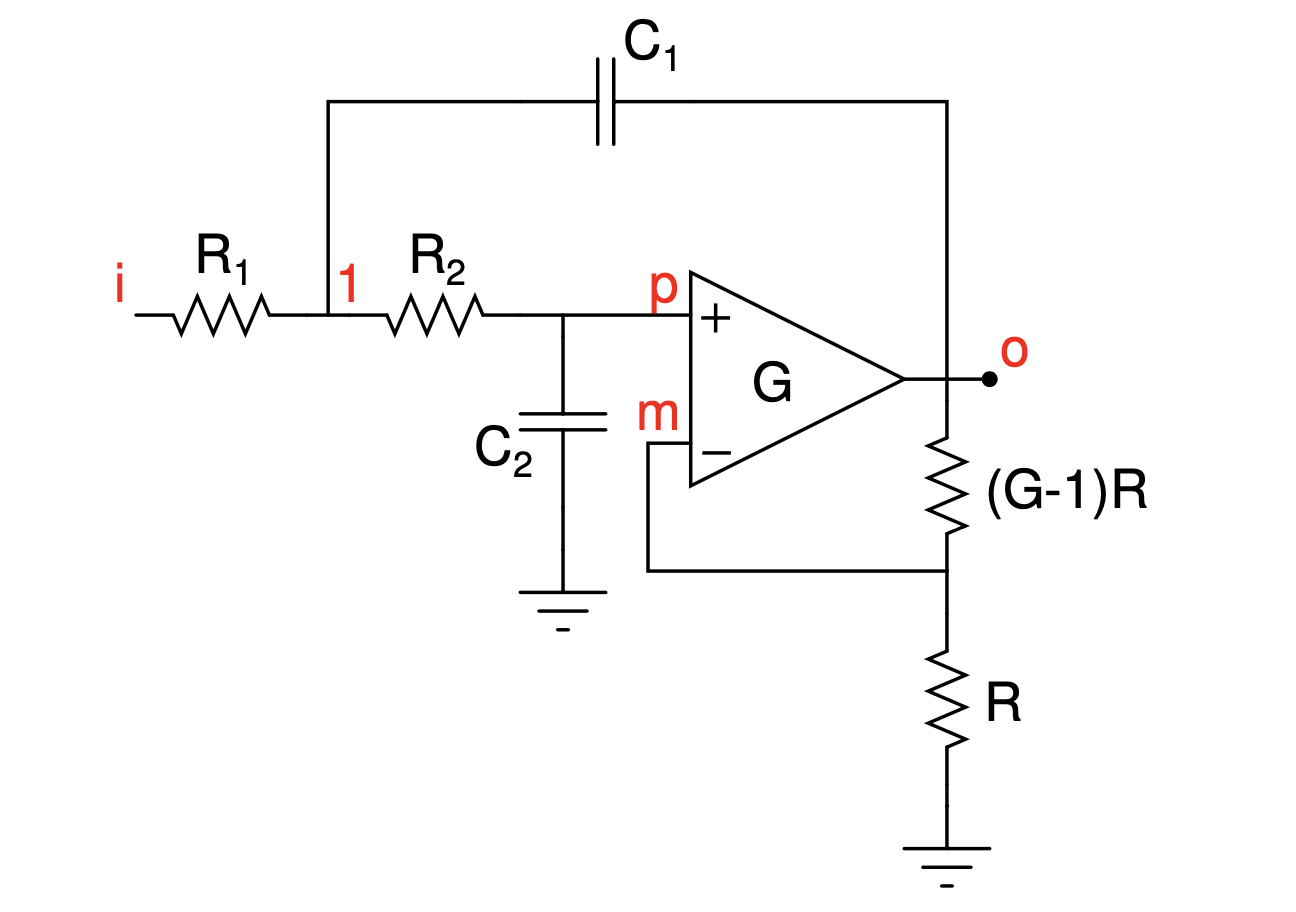
\includegraphics[scale=0.5]{low_pass.png}   
   	\caption{Low Pass Filter Circuit}
   	\label{fig:Figure_1}
   \end{figure}
The above circuit gives the following matrix after simplification of Modified Nodal Equations.
\newline
\begin{equation*}
    \begin{bmatrix}
    0   & 0 & 1  & -1/G \\
    \frac{-1}{sR_2C_2}  & 1 & 0 & 0\\
    0  & -G & G & 1 \\
    \frac{-1}{R_1} - \frac{1}{R_2} - s*C_1 & \frac{1}{R_2} & 0 & sC_1
\end{bmatrix}
\begin{bmatrix}
    V_1\\
    V_p\\
    V_m \\
    V_o
\end{bmatrix}
=
\begin{bmatrix}
    0 \\
    0 \\
    0 \\
    \frac{-V_i(s)}{R_1} \\
\end{bmatrix}
\end{equation*}

\begin{lstlisting}
#KCL for low pass filter
def low_pass_filter(R1=10e3,R2=10e3,C1=1e-9,C2=1e-9,G=1.586,Vi=1):
	s = sympy.symbols('s')
	A = sympy.Matrix([[0,0,1,-1/G],[-1/(1+s*R2*C2),1,0,0], [0,-G,G,1],[-1/R1-1/R2-s*C1,1/R2,0,s*C1]])
	b = sympy.Matrix([0,0,0,-Vi/R1])
	V = A.inv()*b
	return (A,b,V)
\end{lstlisting}

\subsection{Magnitude response}
The magnitude response of the circuit is,
\begin{lstlisting}
A,b,V = low_pass_filter()	#Solve for low pass filter
H_lowpass = V[3]
hf = sympy.lambdify(s,H_lowpass,"numpy")	#Convert transfer function to python function
v = hf(ss)		#Do freq sweep and plot magnitude response
g1 = General_Plotter("frequency$\longrightarrow$","|H(s)|$\longrightarrow$","Bode plot of low pass filter",[],1)
g1.plot_loglog(w,abs(v))
g1.show()
\end{lstlisting}
\begin{figure}[!tbh]
   	\centering
   	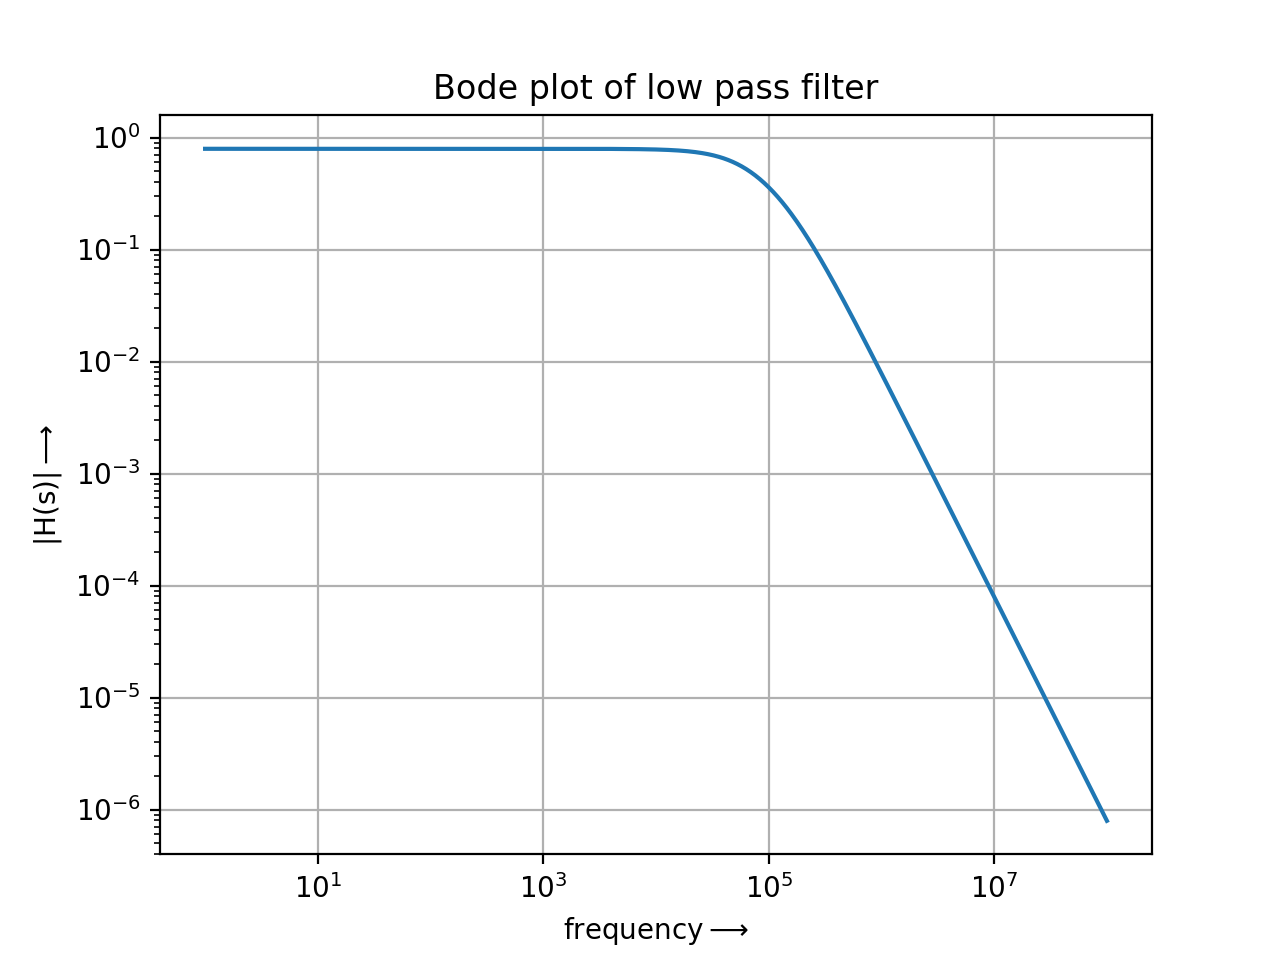
\includegraphics[scale=0.5]{low_pass_bode.png}   
   	\caption{Low pass filter Magnitude response}
   	\label{fig:Figure_1}
\end{figure}
Clearly, the circuit acts as a low pass filter as the magnitude response drops rapidly after a certain frequency.


\section{High Pass Filter}
Consider the circuit below,
\begin{figure}[!tbh]
   	\centering
   	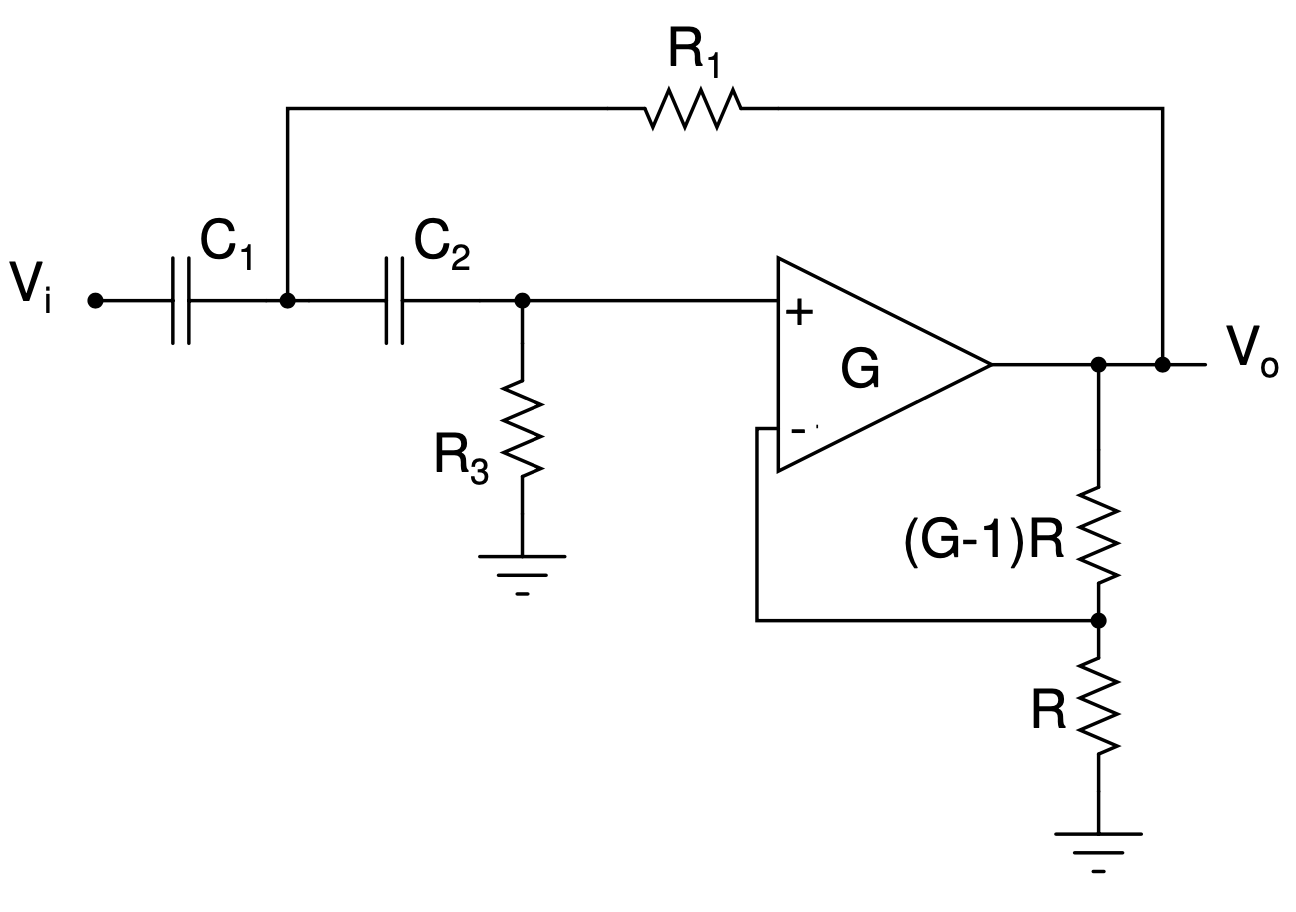
\includegraphics[scale=0.5]{high_pass.png}   
   	\caption{High Pass Filter Circuit}
   	\label{fig:Figure_1}
   \end{figure}
The above circuit gives the following matrix after simplification of Modified Nodal Equations.
\begin{equation*}
    \begin{bmatrix}
    0   & -1 & 0  & 1/G \\
    \frac{s*C_2*R_3}{1+s*C_2*R_3}  & 0 & -1 & 0\\
    0  & G & -G & 1 \\
    -s*C_2 - \frac{1}{R_1} - s*C_1 & 0 & s*C_2 & \frac{1}{R_1}
\end{bmatrix}
\begin{bmatrix}
    V_1\\
    V_p\\
    V_m \\
    V_o
\end{bmatrix}
=
\begin{bmatrix}
    0 \\
    0 \\
    0 \\
    -V_i(s)*s*C_1 \\
    
\end{bmatrix}
\end{equation*}

\subsection{Magnitude response}
The magnitude response of the circuit is,
\begin{lstlisting}
A,b,V = high_pass_filter()	#Solve for high pass filter
H_highpass = V[3]
hf = sympy.lambdify(s,H_highpass,"numpy")		#Convert transfer function to python function
v = hf(ss)		#Do freq sweep and plot magnitude response
g1 = General_Plotter("frequency$\longrightarrow$","|H(s)|$\longrightarrow$","Bode plot of high pass filter",[],2)
g1.plot_loglog(w,abs(v))
g1.show()
\end{lstlisting}
\begin{figure}[!tbh]
   	\centering
   	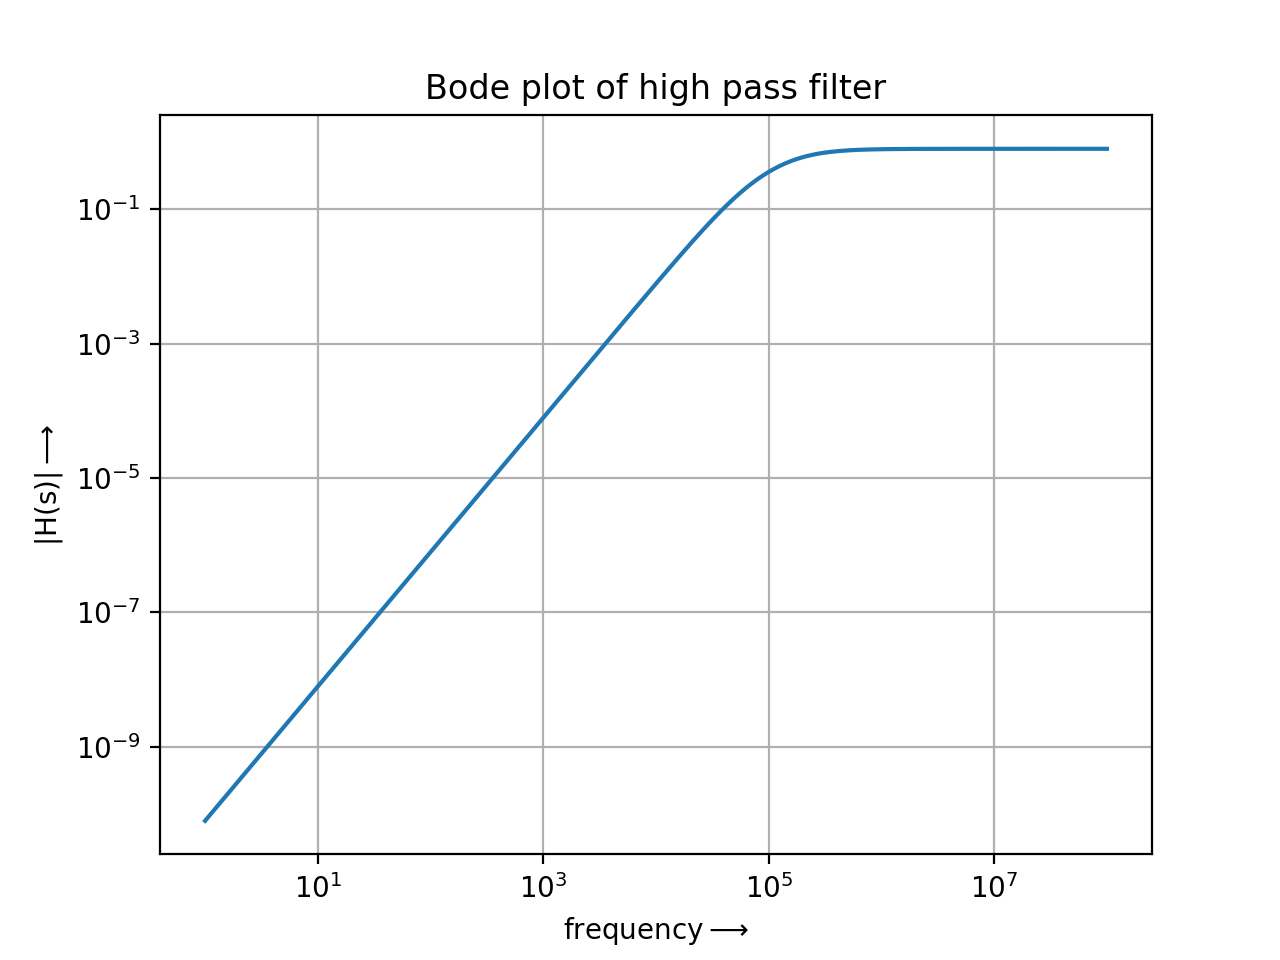
\includegraphics[scale=0.5]{high_pass_bode.png}   
   	\caption{High pass filter Magnitude response}
   	\label{fig:Figure_1}
\end{figure}
Clearly, the circuit acts as a high pass filter as the magnitude response starts with low values and then increases and remains constant with frequency after a certain cut-off frequency.

\section{Converting Sympy to Scipy}
On obtaining the transfer function in it's symbolic representation, we now convert it to a form that can be used by Scipy's Signals package.
\begin{lstlisting}
#Convert transfer function in sympy to scipy
def convert_sympy_to_scipy(H):
	H = sympy.simplify(H)
	n,d = sympy.fraction(H)		#Get numerator and denominator from H
	num,den = sympy.Poly(n,s), sympy.Poly(d,s)	#Convert them into polynomial in 's'
	num,den = num.all_coeffs(), den.all_coeffs()	#Get coefficients of polynomials
	num,den = [float(f) for f in num], [float(f) for f in den]	#Store them in list
	return num,den
\end{lstlisting}

We then use this numerator and denominator coefficients with scipy's various functions to get output for various inputs.

\section{Step Responses}
We now calculate and plot the output for both filters to step input.
\begin{lstlisting}
#Calculate step response to given transfer function in sympy
def step_response(H):
	num,den = convert_sympy_to_scipy(H)		#Sympy to scipy
	den.append(0)							#Multiply H by 1/s for step input
	H = sp.lti(num,den)
	t,x = sp.impulse(H,T = np.linspace(0,1e-3,100000))	#Calculate Impulse response
	return t,x

t,x = step_response(H_lowpass)	#Get stepresponse for low pass filter and plot
g1 = General_Plotter("time$\longrightarrow$","$V_o(t)\longrightarrow$","Step response for low pass filter",[],3)
g1.plot_points(t,x)
g1.show()

t,x = step_response(H_highpass)	#Get stepresponse for high pass filter and plot
g1 = General_Plotter("time$\longrightarrow$","$V_o(t)\longrightarrow$","Step response for high pass filter",[],4)
g1.plot_points(t,x)
g1.show()
\end{lstlisting}

\begin{figure}[!tbh]
   	\centering
   	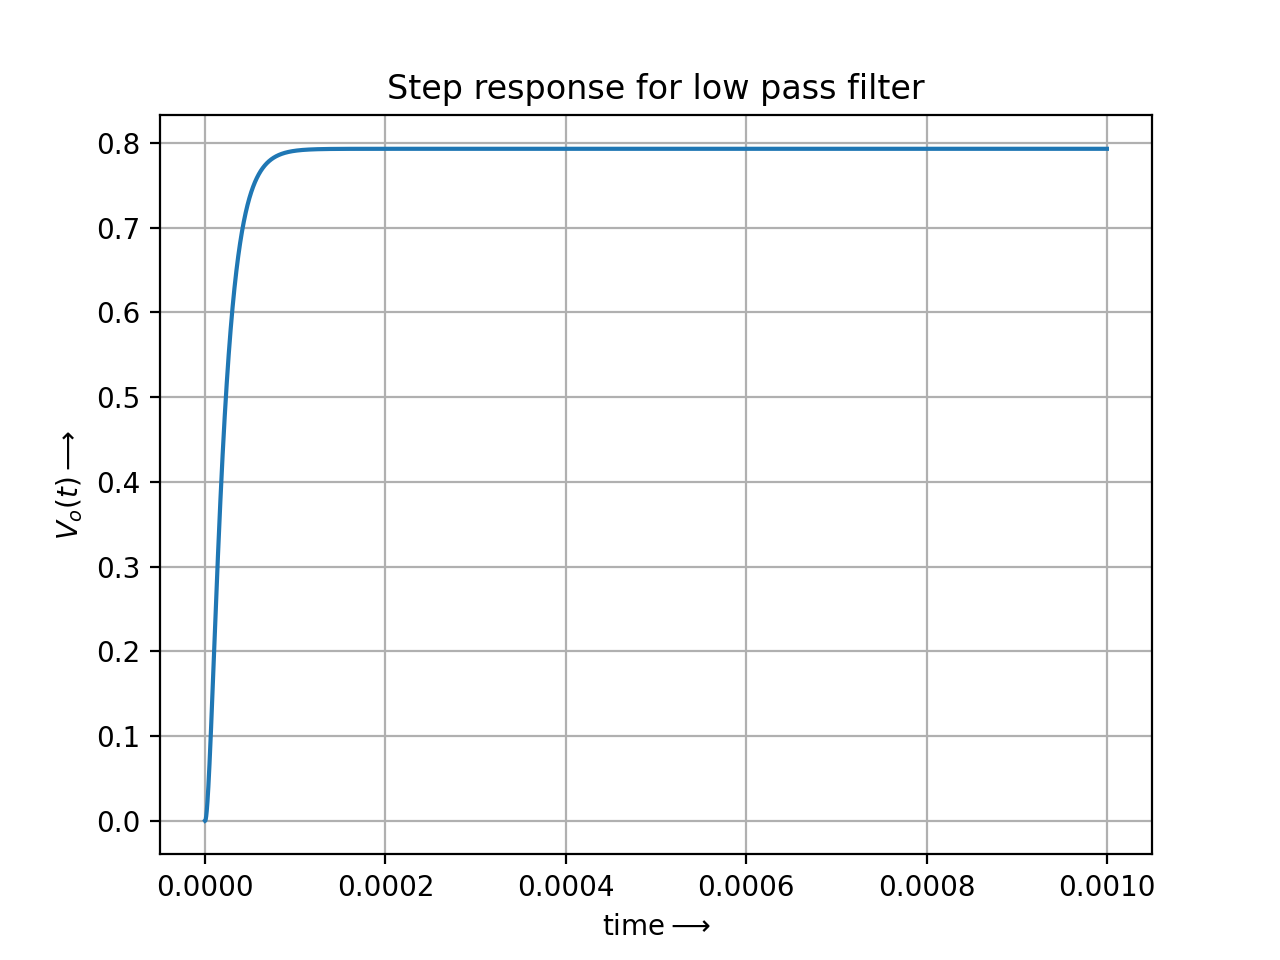
\includegraphics[scale=0.5]{low_pass_step.png}   
   	\caption{Low pass filter step response}
   	\label{fig:Figure_1}
\end{figure}
\newpage
\begin{figure}[!tbh]
   	\centering
   	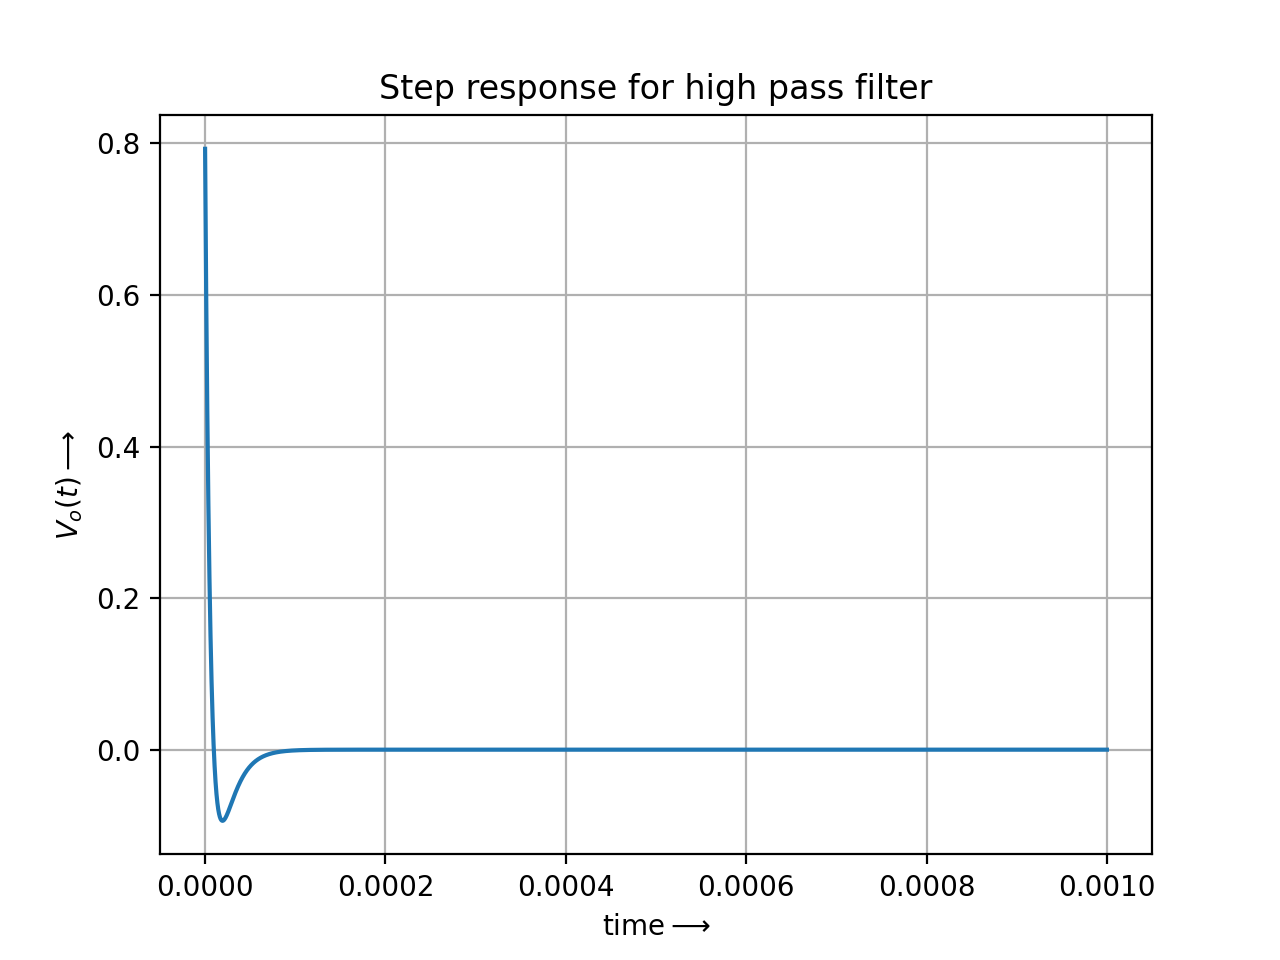
\includegraphics[scale=0.5]{high_pass_step.png}   
   	\caption{High pass filter step response}
   	\label{fig:Figure_1}
\end{figure}
The unit step response,for the high pass filter, as expected is high at t=0 when there is an abrupt change in the input.  For the steady value of the input Vi, the capacitor C1 in the circuit acts as an open switch and allows no current to pass through.  Consequently,  we have a zero voltage at the output node.


\section{Two frequency Sinusoids}
We now plot the output for both the filters corresponding to a input with two sinuoids with one small frequency and one big frequency. The input signal is given by:\\
\begin{center}
$vi = (sin(2000*\pi*t) + cos(2000000*\pi*t))u(t)$
\end{center}

\begin{lstlisting}
#Sum of sinusoids of two frequencies
def sum_of_sinuosids(t):
	return (np.sin(2000*np.pi*t)+np.cos(2e6*np.pi*t))

#Function to calculate output corresponding to given transfer function and input function
def general_input(H,input_time,max_time=1e-3):
	num,den = convert_sympy_to_scipy(H)		#Sympy to scipy
	H = sp.lti(num,den)
	t = np.linspace(0,max_time,100000)		#Time range
	t,y,svec = sp.lsim(H,input_time(t),t)	#Calculate output
	return t,y

#Plotting input signal
t = np.linspace(0,1e-3,1000000)
g1 = General_Plotter("time$\longrightarrow$","$V_i(t)\longrightarrow$","Two frequency signal",[],5)
g1.plot_points(t,sum_of_sinuosids(t))
g1.show()

#Low pass filter on TFS
t1,y1 = general_input(H_lowpass,sum_of_sinuosids)	#Solve for low pass filter
g1 = General_Plotter("time$\longrightarrow$","$V_o(t)\longrightarrow$","Low pass filter on Two frequency signal",[],6)
g1.plot_points(t1,y1)
g1.show()

#High pass filter on TFS
t1,y1 = general_input(H_highpass,sum_of_sinuosids,1e-5)	#Solve for high pass filter
g1 = General_Plotter("time$\longrightarrow$","$V_o(t)\longrightarrow$","High pass filter on Two frequency signal",[],7)
g1.plot_points(t1,y1)
g1.show()
\end{lstlisting}

The input signal along side the output signals are,
\begin{figure}[!tbh]
   	\centering
   	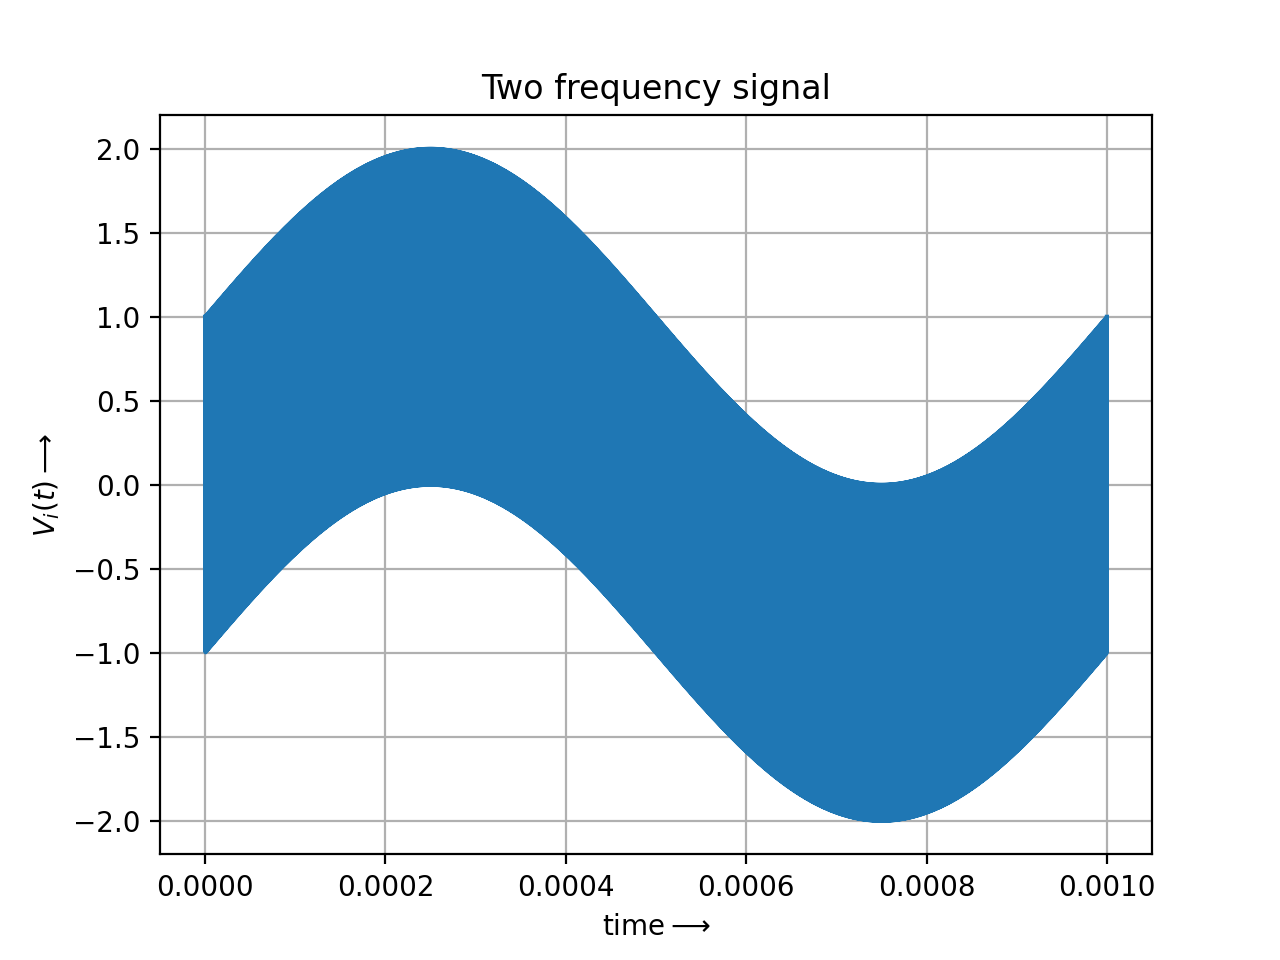
\includegraphics[scale=0.5]{two_freq_input.png}   
   	\caption{Input two frequency sinusoid signal}
   	\label{fig:Figure_1}
\end{figure}
\begin{figure}[!tbh]
   	\centering
   	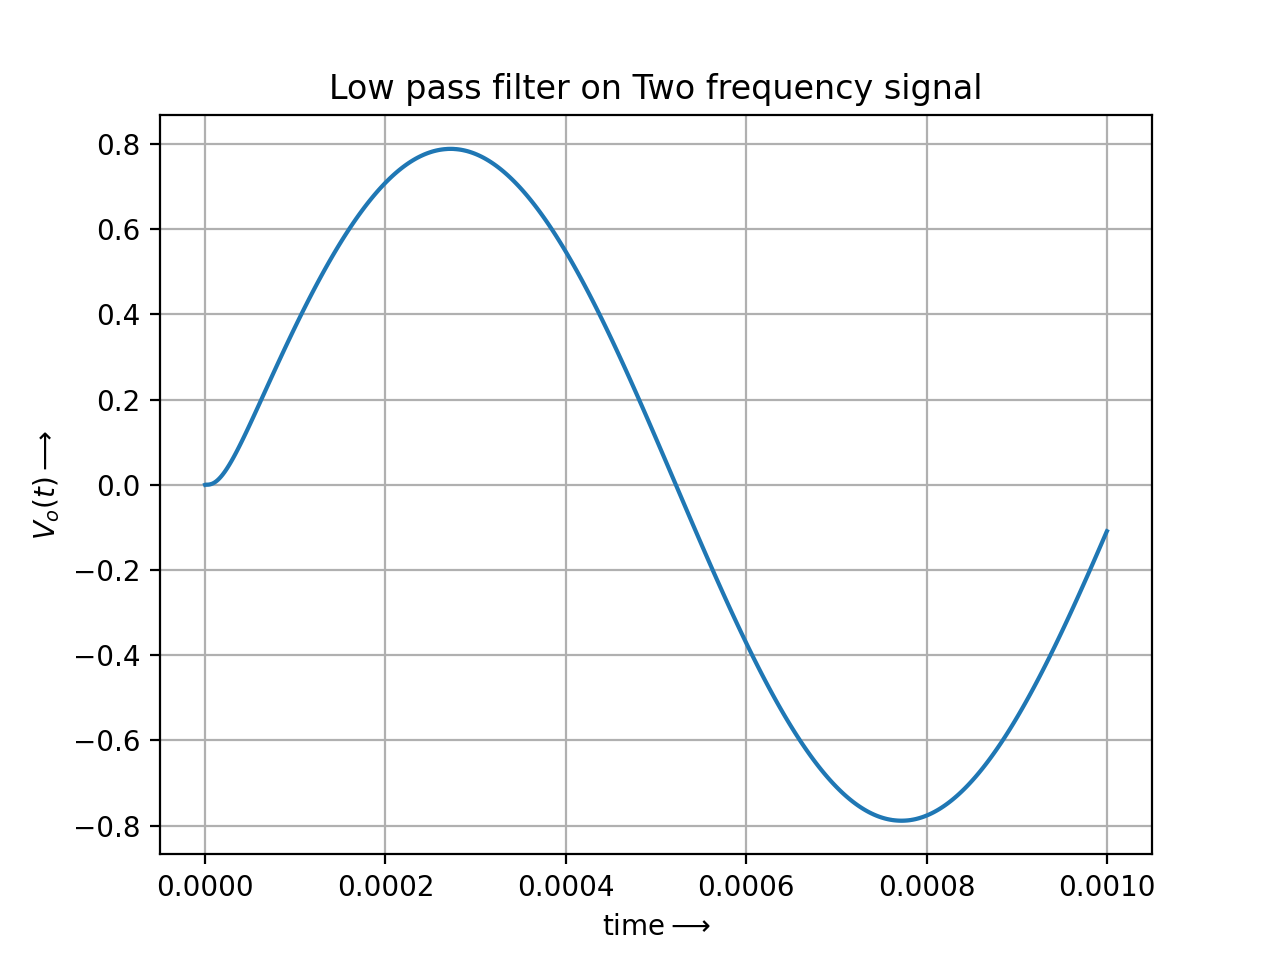
\includegraphics[scale=0.5]{low_pass_tfs.png}   
   	\caption{Low pass filter response}
   	\label{fig:Figure_1}
\end{figure}
We see that the high frequency part of the signal has been attenuated and only the low frequency remains. This is what we expected from a low pass filter.
\begin{figure}[!tbh]
   	\centering
   	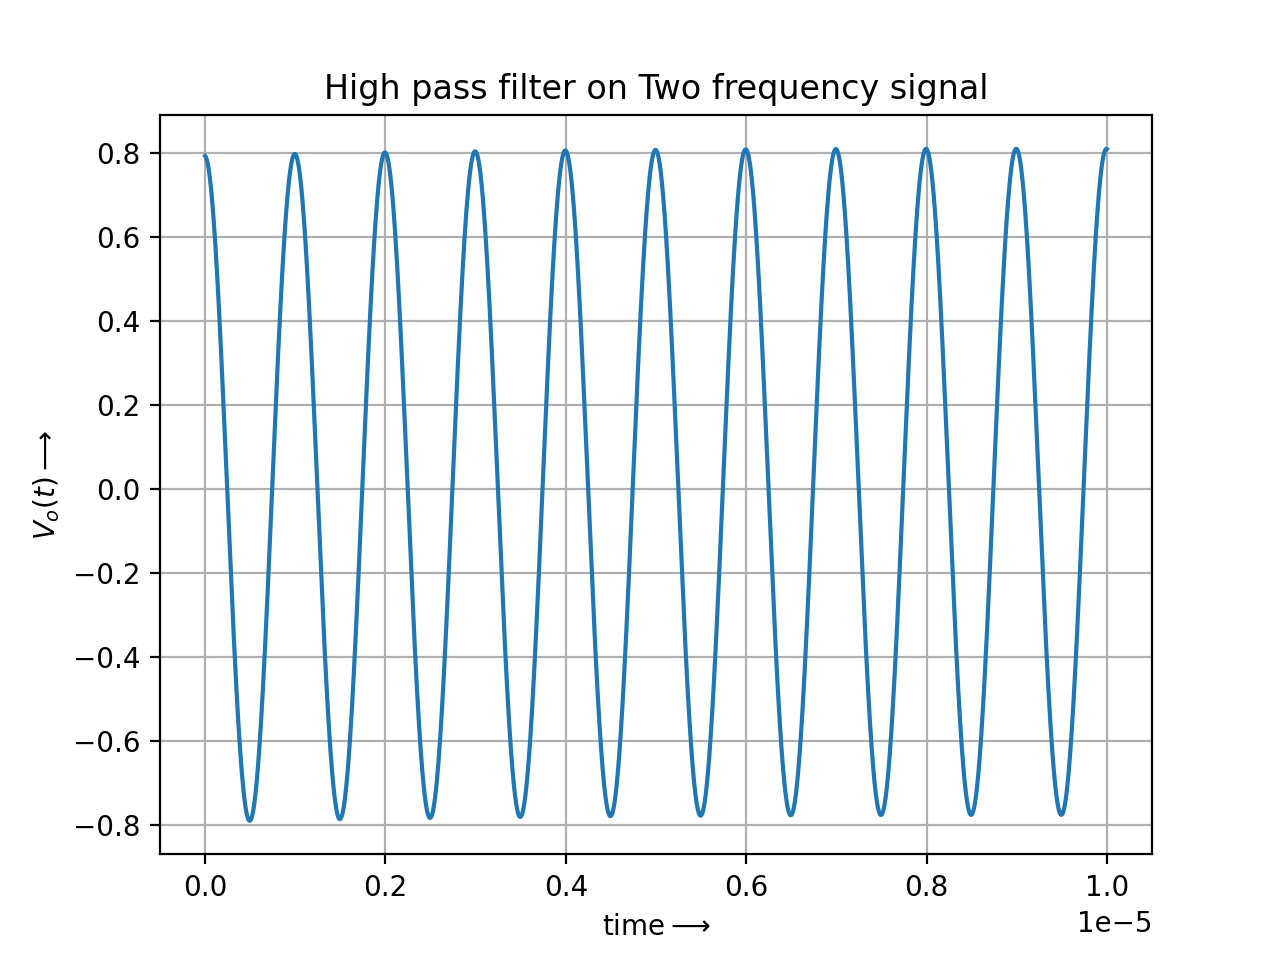
\includegraphics[scale=0.5]{high_pass_tfs.png}   
   	\caption{High pass filter response}
   	\label{fig:Figure_1}
\end{figure}
Similarly for the high pass filter, only the high frequency signal remains while the other gets attenuated. Thus, we can confirm that the cut-off frequencies for both the circuits lie in between the frequencies of the input signal.

\section{Damped Sinusoids}
We now observe and plot outputs to damped sinusoids to different frequencies. Just like the two frequency sinusoids case, we expect the low pass filter to pass low frequency signal while the opposite for high frequency signal.
\subsection{Low frequency damped sinusoid}
The low frequency input signal is,
\begin{equation}
    f(t) = sin(10^3*t)*e^{-10t}
\end{equation}
\begin{lstlisting}
#Low frequency damped sinusoid
def damped2(t,decay=1e1,freq=1e3):
	return np.cos(freq*t)*np.exp(-decay*t) * (t>0)

#Low pass filter on low freq damped
t = np.linspace(0,0.5,1000000)
t3,y3 = general_input(H_lowpass,damped2,0.5)	#Solve for low pass filter
g1 = General_Plotter("time$\longrightarrow$","Voltage$\longrightarrow$","Low pass filter on low freq damped",[],8)
g1.plot_points(t,damped2(t),"Input signal")	#Plotting input signal
g1.plot_points(t3,y3,"Output signal")		#Plotting output signal
g1.show(1)

#High pass filter on low freq damped
t3,y3 = general_input(H_highpass,damped2,0.5)	#Solve for high pass filter
g1 = General_Plotter("time$\longrightarrow$","Voltage$\longrightarrow$","High pass filter on low freq damped",[],9)
g1.plot_points(t,damped2(t),"Input Signal")	#Plotting input signal
g1.plot_points(t3,y3,"Output Signal")		#Plotting output signal
g1.show(1)
\end{lstlisting}
The output for both the filters are,
\begin{figure}[!tbh]
   	\centering
   	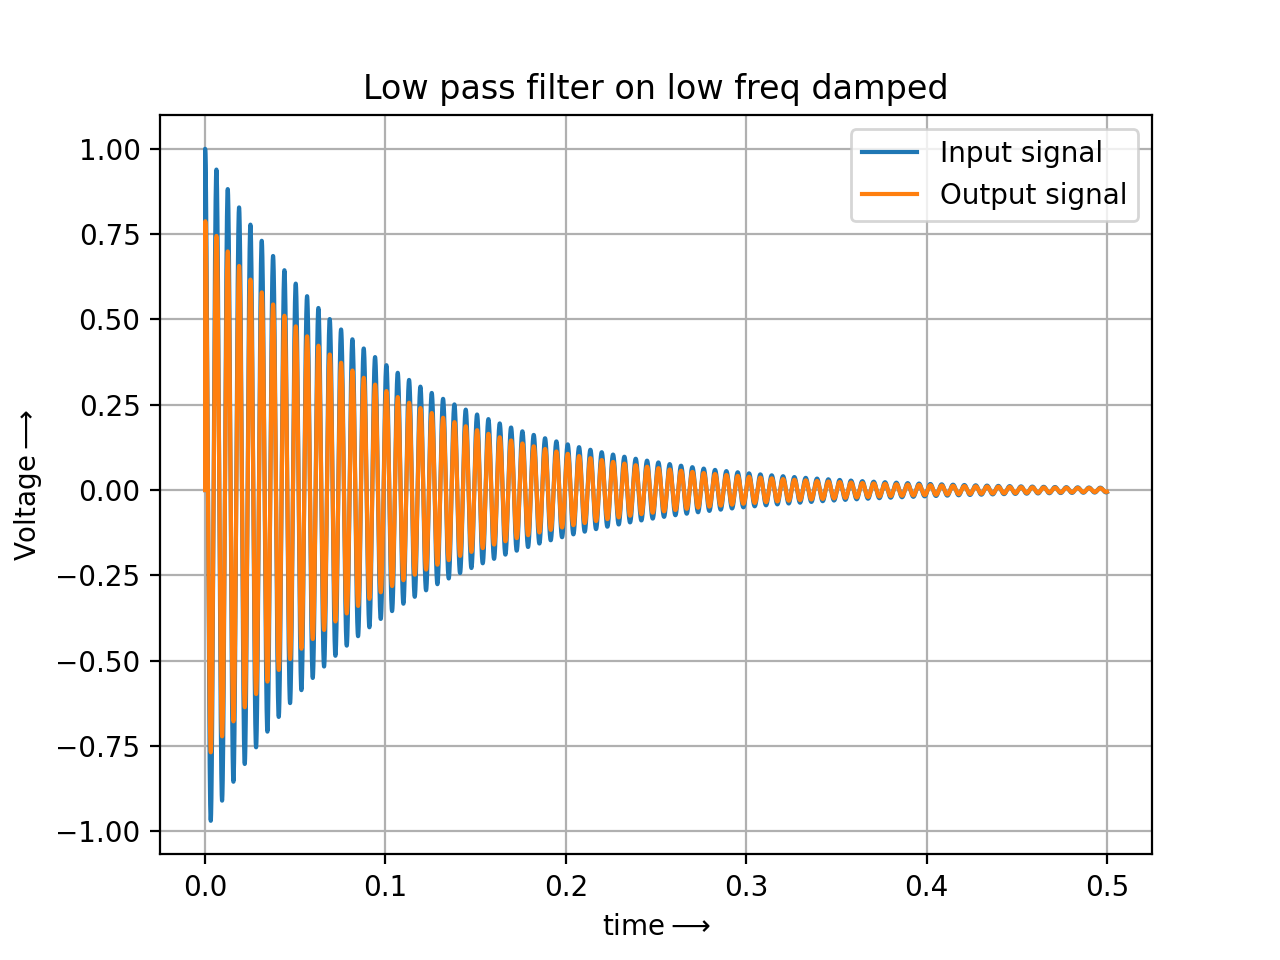
\includegraphics[scale=0.5]{low_pass_low_damped.png}   
   	\caption{Low pass filter response to low freq damped}
   	\label{fig:Figure_1}
\end{figure}
\begin{figure}[!tbh]
   	\centering
   	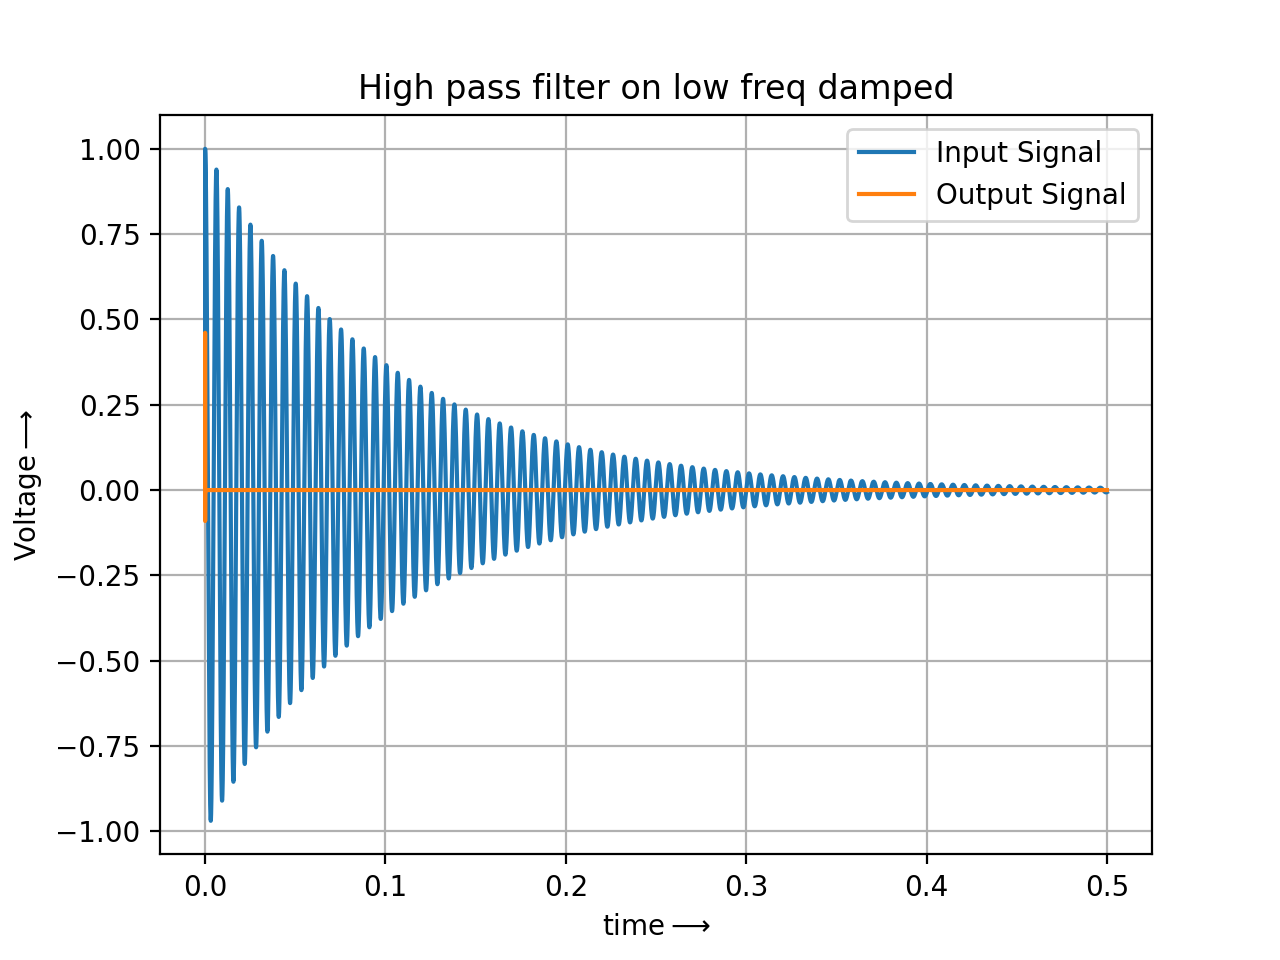
\includegraphics[scale=0.5]{high_pass_low_damped.png}   
   	\caption{High pass filter response to low freq damped}
   	\label{fig:Figure_1}
\end{figure}
Just as expected, the low pass filter allowed the signal to pass while the high pass signal attenuated it.

\subsection{High frequency damped sinusoid}
The high frequency input signal is,
\begin{equation}
    f(t) = sin(10^7*t)*e^{-3*10^3t}
\end{equation}
\begin{lstlisting}
#Low pass filter on high freq damped
t = np.linspace(0,1e-3,1000000)
t2,y2 = general_input(H_lowpass,damped1)	#Solve for low pass filter
g1 = General_Plotter("time$\longrightarrow$","damped$\longrightarrow$","Low pass filter on high freq damped",[],10)
g1.plot_points(t,damped1(t),"Input Signal")	#Plotting input signal
g1.plot_points(t2,y2,"Output Signal")		#Plotting output signal
g1.show(1)

#High pass filter on high freq damped
t2,y2 = general_input(H_highpass,damped1)	#Solve for high pass filter
g1 = General_Plotter("time$\longrightarrow$","damped$\longrightarrow$","High pass filter on high freq damped",[],11)
g1.plot_points(t,damped1(t),"Input Signal")	#Plotting input signal
g1.plot_points(t2,y2,"Output Signal")		#Plotting output signal
g1.show(1)
\end{lstlisting}

The corresponding outputs are,
\begin{figure}[!tbh]
   	\centering
   	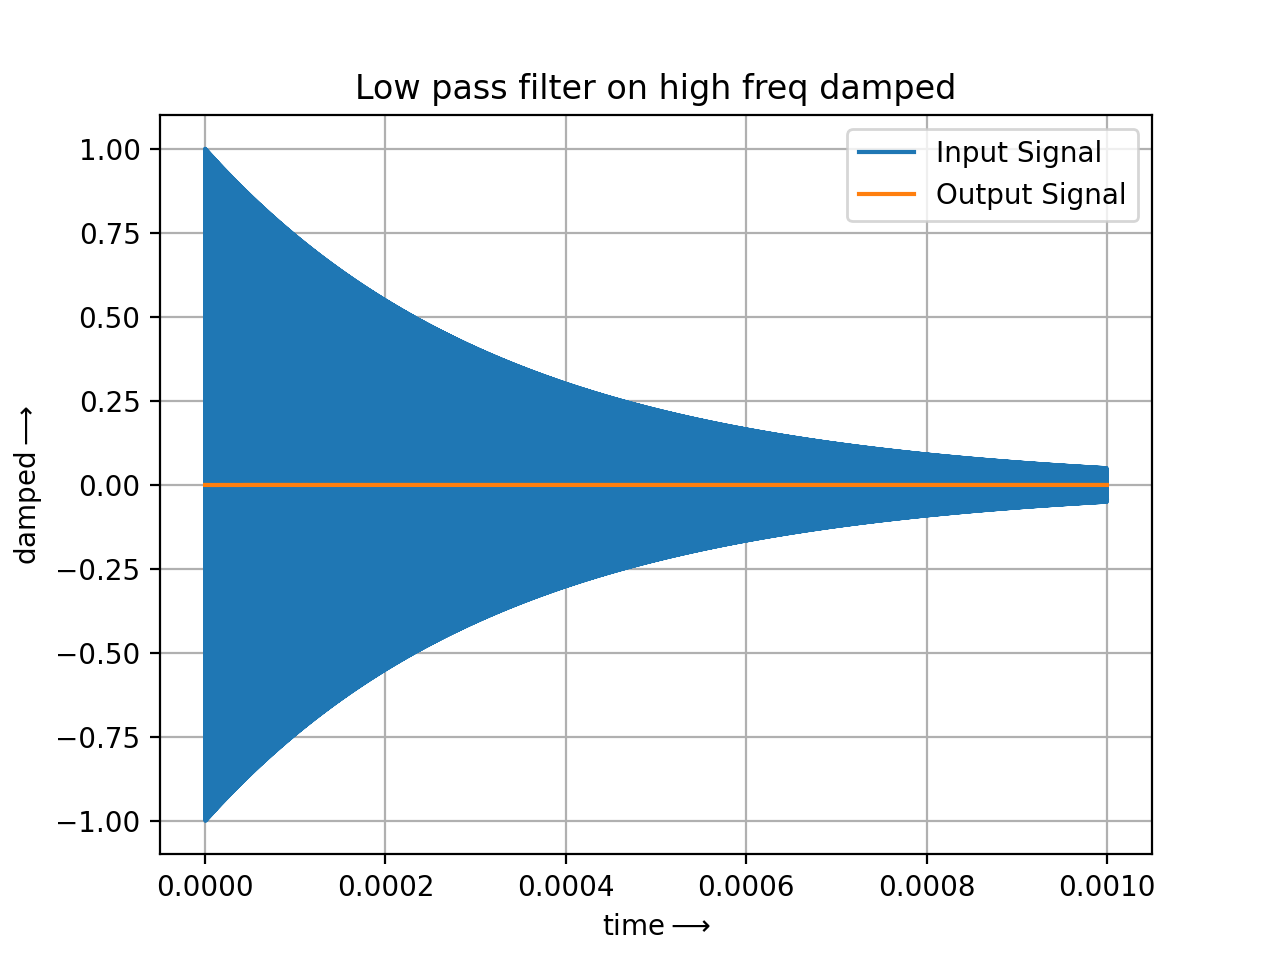
\includegraphics[scale=0.5]{low_pass_high_damped.png}   
   	\caption{Low pass filter response to high freq damped}
   	\label{fig:Figure_1}
\end{figure}
\begin{figure}[!tbh]
   	\centering
   	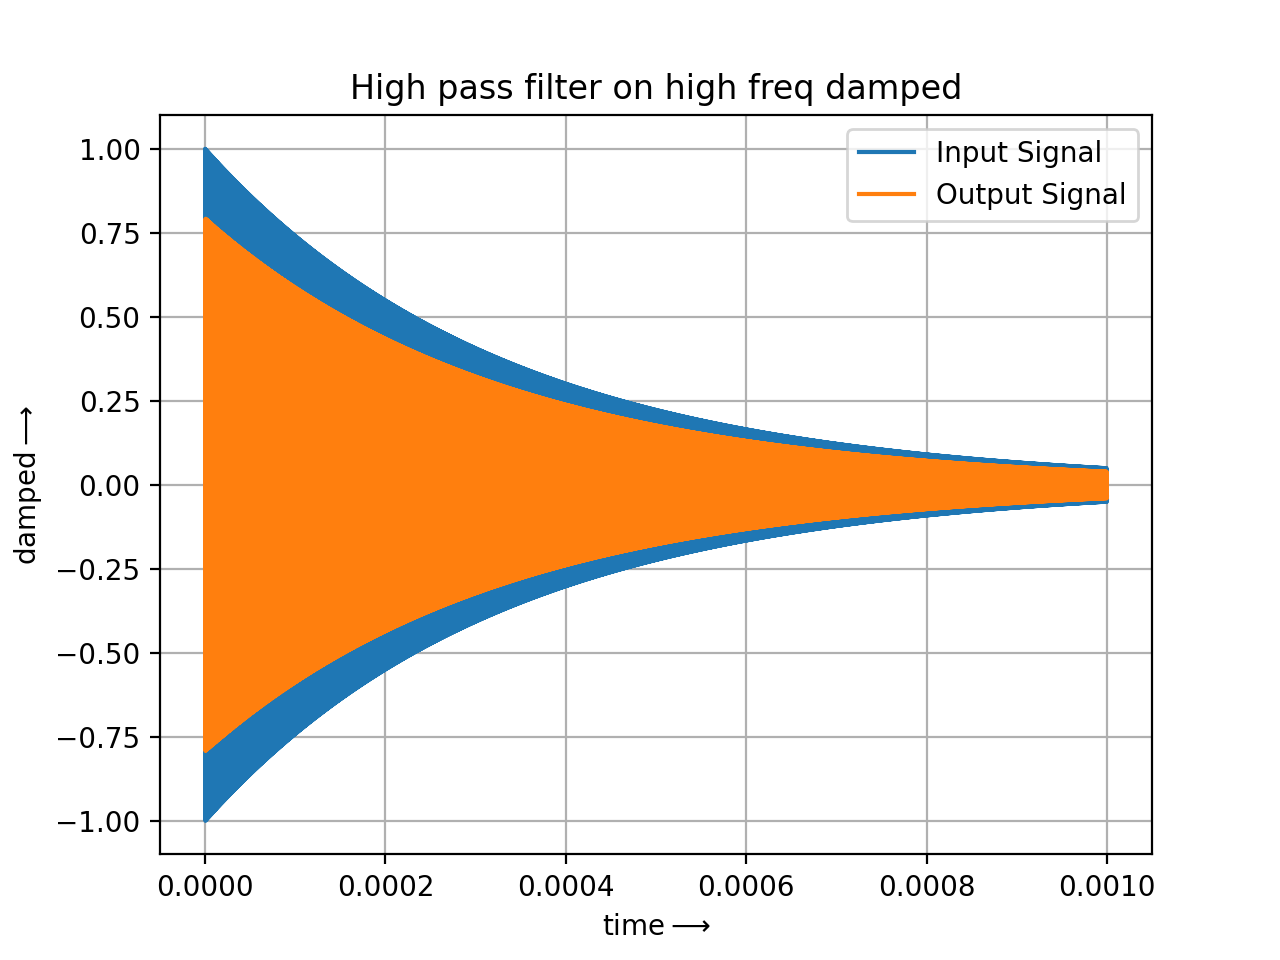
\includegraphics[scale=0.5]{high_pass_high_damped.png}   
   	\caption{Low pass filter response to high freq damped}
   	\label{fig:Figure_1}
\end{figure}
Now, this time as expected the low pass filter attenuated the signal to zero, while high pass filter allowed it to pass.

\newpage
\section{Conclusion}
In conclusion, the sympy module has allowed us to analyse quite complicated circuits by analytically solving their node equations. We then interpreted the circuit behaviour by plotting time domain responses of them to various inputs using the signals toolbox. Thus, sympy combined with the scipy.signal module is a very useful toolbox for analyzing complicated systems like the active filters in this assignment.
\end{document}
